\documentclass[12pt, a4paper]{article}
\usepackage{times}
\usepackage[magyar]{babel}
\usepackage{amsmath}
\usepackage[lmargin = 2.5 cm, tmargin = 2.5 cm, bmargin = 2.5 cm, rmargin = 2.5 cm]{geometry}
\usepackage{t1enc}
\usepackage{fancyhdr}
\usepackage{hyperref}
\usepackage{tabularx}
\usepackage{amsthm}
\usepackage{amssymb}
\usepackage{amsfonts}
\usepackage[usenames,dvipsnames]{xcolor}
\usepackage{float}
\usepackage{graphicx}
\usepackage{listings}
\usepackage{caption}
\usepackage{matlab-prettifier}
\usepackage{varwidth}
\usepackage{setspace}
\usepackage[style=ieee, citestyle=numeric-comp]{biblatex}
\usepackage{csquotes}
\usepackage{multicol}

\addbibresource{irodalomjegyzek.bib}

\begin{document}

\begin{center}
\LARGE\textbf{Hátoldali reflexiós echelon terahertzes forrás optimalizálása numerikus számításokon keresztül}\vspace*{0.7cm}\\\large
Illés Gergő $^{1,*}$, Krizsán Gergő $^{1,2}$, Pálfalvi László $^1$, Tibai Zoltán $^1$, Almási Gábor $^1$, Hebling János $^{1,2,3}$, Tóth György $^1$\vspace*{0.4cm}\\\normalsize
\textit{$^1$ Pécsi Tudományegyetem, Fizikai Intézet, Pécs, Magyarország\\
$^2$ Szentágothai János Kutatóközpont, Pécs, Magyarország\\
$^3$ ELKH-PTE ?Nagy Térerősségű Terahertzes Kutatócsoport?, Pécs, Magyarország\\
$^*$ illesg@gamma.ttk.pte.hu}
\end{center}\vspace*{0.5cm}
\begin{abstract}\noindent
Az optikai terahertzes források fejlődésével lehetőség nyílt arra, hogy 1 mJ nagyságrendű impulzusenergiákat állítsunk elő \cite{wu20201}. Ezt az impulzusenergiát a döntött impulzusfrontú gerjesztés módszerét \cite{hebling2002velocity} használva sikerült elérni. Azonban a döntött impulzusfrontú gerjesztés módszerének számos korlátozó tényezője van. Az első, hogy a kristály nagy ékszöggel rendelkezik, a második, hogy a nagy impulzusfront-döntés következtében a pumpaimpulzus nagymértékű szögdiszperzióval rendelkezik, a harmadik pedig, hogy az elrendezésben használt leképző rendszer nem tökéletes, leképzési hibák keletkeznek. Ezen hibák enyhítésére lehetőséget ad a hátoldali reflexiós elrendezés \cite{krizsan2020lithium,toth2019single}. A Pécsi Terahertzes kutatócsoport már végzett számításokat az elrendezésen, azonban az akkor használt modell nem vette figyelembe a terahertzes impulzus visszahatását a pumpaimpulzusra.
\end{abstract}
\onehalfspace
\section{Az elrendezés vázlata}
A hátoldali reflexiós echelon elrendezés sematikus ábráját az 1. ábra mutatja be.
\begin{figure}[H]
\centering
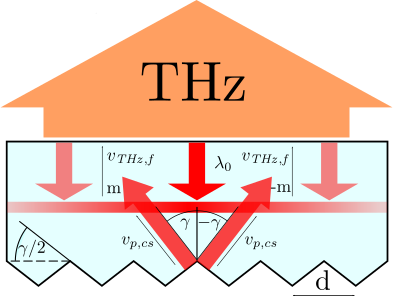
\includegraphics[width=0.7\textwidth]{rajz-1.pdf}
\caption{A hátoldali reflexiós echelon sematikus ábrája \cite{toth2019single}}
\end{figure}
Az elrendezés úgy működik, hogy a pumpaimpulzus a kristályra merőlegesen lép be, majd a kristály hátoldalához érve, a megmunkált felületen diffraktálódik. Ezen megmunkálásnak olyannak kell lennie, diffrakció következtében a kialakuló impulzusfrontdöntés megfeleljen a sebességillesztési feltételnek \cite{hebling2002velocity}. Amennyiben ez teljesül úgy hatékonyan fog keletkezni a terahertzes (továbbiakban THz-es) impulzus. Az keletkező THz-es impulzus a kristály belépő felületén fog távozni, haladási iránya pedig merőleges lesz erre a felületre, aminek következtében nagy hatásfokú lesz a kicsatolás. 
\section{Numerikus modell}
A számítások olyan numerikus modellel készültek amelyek figyelembe veszik a THz-es impulzus visszahatását a pumpaimpulzusra \cite{ravi2014limitations}. A döntött impulzusfrontú gerjesztési technika modellezésénél azt tapasztaltuk, hogy a visszahatás következtében nagy mértékben csökken az elérhető maximális térerősséget, valamint azt, hogy azon kristályhossz ahol a hatásfok maximális rövidebb lesz. További számolások során megállapítottuk, hogy a maximális hatásfokhoz tartozó kristályhosszt túllépve a THz-es impulzus megszűnik egyciklusúnak, a térerősségének maximuma nagymértékben csökken és ezáltal használhatatlanná válik. Az itt bemutatott eredményeket a \cite{ravi2014limitations}-ben bemutatott modell módosított változatával kaptuk.
\section{Eredmények}
\singlespace
\printbibliography[title = Irodalomjegszék]
\end{document}